

In the registration process, the metric typically compare intensity values 
in the fixed image with the corresponding values in the transformed moving
image. When a point is mapped from one space to another by a transform,
it will in general be mapped to a non-grid position. Therefore, interpolation
is required to evaluate the image intensity at the mapped position.

\begin{figure}
\center
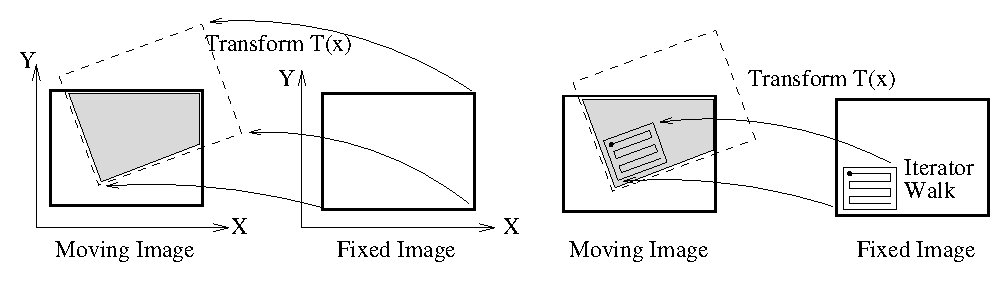
\includegraphics[height=6cm]{ImageOverlap.eps}
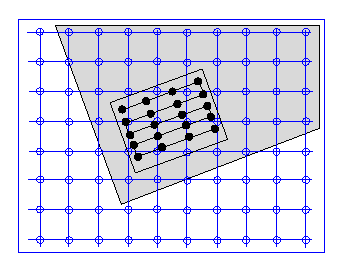
\includegraphics[height=6cm]{ImageOverlapInterpolator.eps}
\caption{ The moving image is mapped into the fixed image space under some spatial
transformation. Grid positions of the fixed image maps to non-grid positions of the
moving image. Interpolation is needed for estimating the intensity of the
moving image at these non-grid positions.}
\label{fig:ImageOverlapInterpolator}
\end{figure}

ITK currently offers three different interpolation schemes: nearest-neighbor,
linear and B-Spline. In the context of registration, the interpolation method
affects the smoothness of the optimization search space and the overall
computation time. On the other hand, interpolations are executed thousands of
times in a single optimization cycle. Hence, the user has to tradeoff the
simplicity of computation with smoothness when selecting the interpolation 
scheme.

 
\subsection{Nearest Neighbor Interpolation}
\label{sec:NearestNeighborInterpolation}
%Use the intensity of the nearest grid point
%Cheap, piecewise constant with jump at grid points

\subsection{Linear Interpolation}
\label{sec:LinearInterpolation}
%Assumes intensity varies linear between grid points.
%More expensive than nearest neighbor, continuous intensity
%by distcontinous gradient

\subsection{B-Spline Interpolation}
\label{sec:BSplineInterpolation}
%Over and undershoots
%Mirror boundary
%Order 0 to 5
%Smoothest, most computation


